\documentclass[10pt]{ps-exercise}
\usepackage{float}
\author{Raphael Gwiggner and Christoph Sch\"opf}
\date{\today}
\subject{Distributed Systems}
\title{Sheet 02}

\begin{document}
\section{Protocol}
\begin{quote}
All required messages: \\ \\
Client:
\begin{itemize}
\item Username
\item "1" for Addition
\item "2" for Subtraction
\item "3" for Multiplication
\item "4" for Factorial
\end{itemize}
Server:
\begin{itemize}
\item Login succesful?
\item Result
\end{itemize}
\end{quote}
\begin{figure}[H]
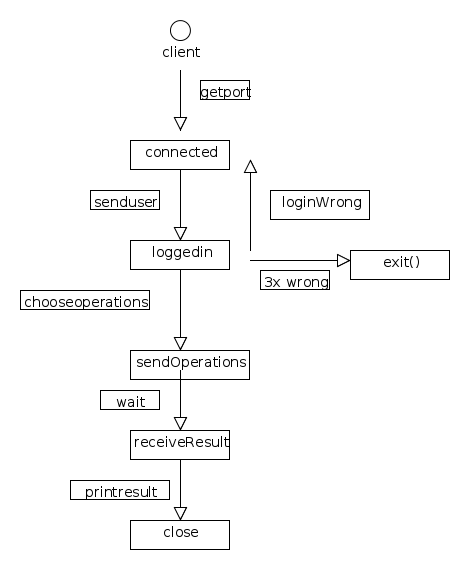
\includegraphics[scale=0.6]{client.png}
\end{figure}
\begin{figure}[H]
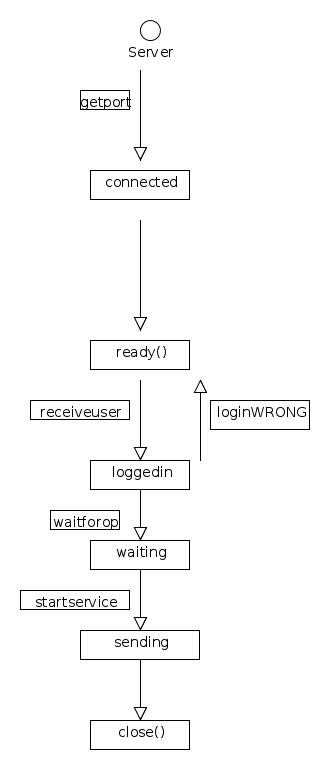
\includegraphics[scale=0.6]{server.png}
\end{figure}
\end{document}